\documentclass{article}

% if you need to pass options to natbib, use, e.g.:
% \PassOptionsToPackage{numbers, compress}{natbib}
% before loading nips_2016
%
% to avoid loading the natbib package, add option nonatbib:
% \usepackage[nonatbib]{nips_2016}

\usepackage[final]{nips_2016}

% to compile a camera-ready version, add the [final] option, e.g.:
% \usepackage[final]{nips_2016}

\usepackage[utf8]{inputenc} % allow utf-8 input
\usepackage[T1]{fontenc}    % use 8-bit T1 fonts
\usepackage{hyperref}       % hyperlinks
\usepackage{url}            % simple URL typesetting
\usepackage{booktabs}       % professional-quality tables
\usepackage{amsfonts}       % blackboard math symbols
%\usepackage{nicefrac}       % compact symbols for 1/2, etc.
\usepackage{microtype}      % microtypography

\usepackage{amssymb, amsmath}
\usepackage{epsfig}
\usepackage{array}
\usepackage{ifthen}
\usepackage{color}
\usepackage{fancyhdr}
\usepackage{graphicx}
\usepackage{mathtools}
\usepackage{csquotes}
\usepackage{xcolor}
\usepackage{multirow}
\newcommand\crule[3][black]{\textcolor{#1}{\rule{#2}{#3}}}

\newcommand{\tr}{\text{tr}}
\newcommand{\E}{\textbf{E}}
\newcommand{\diag}{\text{diag}}
\newcommand{\argmax}{\text{argmax}}
\newcommand{\Cov}{\text{Cov}}
\newcommand{\Var}{\text{Var}}
\newcommand{\argmin}{\text{argmin}}
\newcommand{\Vol}{\text{Vol}}
\newcommand{\comm}[1]{}
\newcommand{\indep}{\rotatebox[origin=c]{90}{$\models$}}
\newcommand{\Cor}{\text{Cor}}

\definecolor{color1}{RGB}{128,13,13}
\definecolor{color2}{RGB}{70,128,13}
\definecolor{color3}{RGB}{13,128,128}
\definecolor{color4}{RGB}{70,13,128}

\title{How many faces can be recognized? Performance extrapolation for
  multi-class classification}

% The \author macro works with any number of authors. There are two
% commands used to separate the names and addresses of multiple
% authors: \And and \AND.
%
% Using \And between authors leaves it to LaTeX to determine where to
% break the lines. Using \AND forces a line break at that point. So,
% if LaTeX puts 3 of 4 authors names on the first line, and the last
% on the second line, try using \AND instead of \And before the third
% author name.

\author{
  Charles Y.~Zheng \\
  Department of Statistics\\
  Stanford University\\
  Stanford, CA 94305 \\
  \texttt{snarles@stanford.edu} \\
  %% examples of more authors
  \And
  Rakesh ~Achanta \\
  Department of Statistics\\
  Stanford University\\
  Stanford, CA 94305 \\
  \texttt{rakesha@stanford.edu} \\
  \And
  Yuval ~Benjamini \\
  Department of Statistics \\
  Hebrew University\\
  Jerusalem, Israel\\
  \texttt{yuval.benjamini@mail.huji.ac.il}
  %% Address \\
  %% \texttt{email} \\
  %% \AND
  %% Coauthor \\
  %% Affiliation \\
  %% Address \\
  %% \texttt{email} \\
  %% \And
  %% Coauthor \\
  %% Affiliation \\
  %% Address \\
  %% \texttt{email} \\
  %% \And
  %% Coauthor \\
  %% Affiliation \\
  %% Address \\
  %% \texttt{email} \\
}

\begin{document}
% \nipsfinalcopy is no longer used

\maketitle

\begin{abstract}
The difficulty of multi-class classification generally increases with
the number of classes.  \emph{Recognition systems} employ such
classifiers in order to recognize people, spoken words, or chemicals:
it is often of interest to know how many species the system can be
trained to recognize before dropping below a minimum accuracy
threshold.  However, before such systems are deployed, typically only
a small number of species are available for testing the system.  Can
we predict how well the recognition system will scale with an
increased number of classes?  We define a class of
\emph{asymptotically generative} classifiers, which include
$k$-nearest neighbors, multinomial regression, one-vs-one and
one-vs-all classifiers: for recognition systems based on such
classifiers, the problem of predicting scalability reduces to the
problem of estimating the higher-order moments of a \emph{conditional
  accuracy distribution}, which in turn can be estimated from data.
\end{abstract}

\section{Introduction}

Object recognition, face recognition (or more generally person
recognition) and language are a few of the cognitive building blocks
which are fundamental to human cognition, and which can be understood
as examples of generalized classification tasks. Machine
classification can be employed to mimic this power of recognition.  A
robot equipped with a camera can algorithmically segment its input
image into objects, and to learn to recognize unique objects and
people which regularly appear in its environment.  A general approach
to implement such a recognition ability starts by employing some
parametric featurization of the object to be identified.  For example,
for the task of face recognition, one might define features such as
the proportions between the eyes and the relative position and size of
the nose.  The full domain of the recognition task is a collection of
\emph{measurements} (e.g. photographs of faces) which are associated to different
\emph{species.}  The recognition system can be implemented by training
a multi-class classifier to assign measurements to their corresponding
species.  While the system is in deployment, new species may be added
to the system: when this happens, the classifier is retrained (or
updated) using training data from the species to be added.

A limitation to such recognition systems, whether they be natural or
artificial, is that the performance of the system (in terms of correct
classification) can degrade if there are too many species.  A face
recognition algorithm can have very high success rate if it only needs
to distinguish between 100 different faces, but its identifications
may be less reliable when it needs to distinguish between 10000
different faces.  The consequences of such errors may be severe: Cole
(2005) lists 22 cases of fingerprint misindentification in criminal
trials.

Therefore, in the case of engineering recognition systems, it is of
much practical interest to be able to evaluate the reliability of such
systems before they are deployed.  Yet, during the development phase,
typically data from only a fraction of the species in the domain are
available.  From the empirical performance of the classifier on this
initial subset of species, can we predict the performance of the
system on a larger subset of species (or the entire domain)?

A related problem arises in studying \emph{naturally occurring}
recognition systems: for instance, human memory.  Neuroscientists may
be directly interested in the number of different cues which can be
recalled by a subject.  A similar dilemma arises, where data from only
small number of species can be obtained, due to experimental
constraints.  From this data, can we predict the number of species
which can be distinguished by the recognition system, above a minimum
accuracy threshold?

We address this problem of \emph{performance extrapolation} under the
assumption that the initial subset of species is an i.i.d. sample from
a larger population of species.  Section 2 formalizes the recognition
problem, and section 3 formalizes the problem of performance
extrapolation.  For a restricted family of
classifiers--\emph{separable} classifiers, we show that the problem of
performance extrapolation reduces to a problem of nonparametric moment
estimation.  In section 4, we explore methods for nonparametric
estimation.  We propose a method called \emph{moment-constrained
  maximum pseudolikelihood}, and demonstrate that it has reasonable
performance in simulated and real data examples in section 5; section
6 concludes.


\section{The recognition problem}

In the recognition problem, there exists a large or infinite
population of \emph{species}, e.g. individuals, and an infinite
population of \emph{measurements}, and each measurement is associated
with a single species.  A recognition system is an algorithm which
contains a database of measurements from a number of species: each
measurement is represented within the recognition system by a real
vector $y \in \mathbb{R}^p$ which lies in the space $\mathcal{Y}$, and
labeled with an integer-valued ID key.  The ID key is the recognition
system's internal representation of the species associated to the
measurements: we assume that the database has the property of
\emph{integrity}, where any two measurements in the database share the
same ID key if and only if they are associated with the same species.
Given a query measurement, the system answers with an ID number: this
answer is correct if and only if the query measurement and the
database measurements labeled with the same ID are associated to the
same species.  Without loss of generality, take the ID keys to be
$\{1,2,\hdots, k\}$, and let $y^{(i), j}$ denote the $j$th measurement
associated with ID key $i$ in the database; let $n_i$ be the number of
measurements associated to the $i$th ID key, and $n = \sum_{i=1}^k
n_i$ be the total number of measurements.

The recognition system maps queries $y$ to an ID key; let us refer to
this mapping as $f:\mathcal{Y} \to \{1,\hdots, k\}$.  New data can be
added to the recognition system over time; we assume it is done in a
manner so that the integrity of the database is preserved.  Let $t =
1, 2 ,\hdots$ refer to discrete time stages, and let $k_t$ denote the
number of classes in the database at time $t$, and $f_t$ denote the
mapping from queries to answers at time $t$; also define $n_{i, t}$
analogously.

\subsection{Multi-class classification}

A natural approach for implementing a recognition system is through
\emph{supervised learning}: the data is input into a supervised
learning algorithm in order to \emph{learn} a classification rule
$f(y)$.  Examples of multi-class classifiers include $k$-nearest
neighbors, multinomial logistic regression, linear discriminant
analysis (LDA), quadratic discriminant analysis (QDA), decision trees,
and random forests, as well as the two `divide and conquer'
approaches, one-vs-one (OVO) and one-vs-all (OVA) (Friedman et al,
2008.)  A unified definition of a classifier is as follows: a
$k$-class classifier $\mathcal{C}$ is a function which takes $k+2$
arguments: the first $k$ arguments are \emph{probability
  distributions} $F_1,\hdots, F_k$, the $(k+1)$st argument is a vector
of prior probabilities $\vec{\pi}$, and the $(k+2)$nd argument is a
\emph{query} $y$
\footnote{We treat randomized classifiers (such as random forests) as
  a probability distribution over deterministic classifiers.}.  The
level sets $\{y: \mathcal{C}(F_1,\hdots, F_k, y) = k\}$ are called
\emph{decision regions.}  We say the classifier is \emph{continuous}
if and only if the \emph{decision regions} of $\mathcal{C}$ are
continuous in the first $k$ arguments with respect to the topology of
weak convergence\footnote{We say that a randomized classifier is
  continuous if and only if it is continuous with probability one.}.
Most of the commonly used classifiers satisfy this definition of
continuity: an exception is $k$-nearest neighbors with fixed $k$, but
then again, $k$-nearest neighbors with $\lim_{n \to \infty} k/n \in
(0, 1)$ is continuous.  \emph{Training a classifier} refers to
defining a classification rule
\[
f(y) = \mathcal{C}(\hat{F}_1,\hdots, \hat{F}_k, \vec{\pi}, y)
\]
where $\hat{F}_i = \frac{1}{n_i}\sum_{j=1}^{n_i} \delta_{y^{(i), j}}$
is the empirical distribution, and where $\vec{\pi}$ is commonly set
to either be the uniform distribution on $k$ elements, or the
empirical proportions of the classes, but can be adjusted in order to
favor certain classes over others.

Whenever new data is added, the classifier is retrained.  
Let $\hat{F}_{i, t}$ denote the empirical distribution of the
measurements of species $i$ at time $t$, and $\hat{F}_t$ denote the
empirical distribution of all measurements at time $t$.

\subsection{Exchangeability}

A key assumption for our theory is that the marginal distributions of
the classes $F_1, F_2, \hdots$ are \emph{exchangeable}: equivalently,
that there exists a measure $\mathbb{F}$ on probability distributions
in $\mathcal{Y}$, and $F_i \sim{i.i.d.} \mathbb{F}$ for $i =
1,\hdots$.  We call $\mathbb{F}$ a meta-distribution.

[[Discuss the signficance of this assumption.  Without it, extrapolation is impossible.]]

\subsection{Asymptotic Generative}

Define a generative classifier $\mathcal{C}$ as satisfying
 \[
\mathcal{C}(F_1,\hdots, F_k, \vec{\pi}, y) = \argmax_i \mathcal{Q}(F_i, \vec{\pi}_i, y).
\]
where $\mathcal{Q}$ is \emph{scoring rule}: a real-valued function
which takes three arguments: a distribution $F$ on $\mathcal{Y}$, a
prior probability $\pi$, and a query measurement $y \in \mathcal{Y}$.
For notational convenience, we assume that ties occur with probability
zero: that is, $\mathbb{F}$ and $\mathcal{Q}$ jointly satisfy the
\emph{tie-breaking} property: for any $\pi \in [0,1]$, letting
$\hat{F}$ be an empirical distribution of finitely many points drawn
from $F \sim \mathbb{F}$ respectively, $Y, Y' \stackrel{iid}{\sim} F$,
\begin{equation}\label{eq:tie}
\Pr[\mathcal{Q}(\hat{F}, \pi, Y) = \mathcal{Q}(\hat{F}, \pi, Y')] = 0.
\end{equation}
Quadratic discriminant analysis and Naive Bayes are two examples of
generative classifiers.  For QDA, the scoring rule is given by
\[
\mathcal{Q}_{QDA}(F, \pi, y) = -(y - \mu(F))^T \Sigma(F)^{-1} (y-\mu(F)) - \log\det(\Sigma(F)) + 2\log\pi
\]
where $\mu(F) = \int y dF(y)$ and $\Sigma(F) = \int (y-\mu(F))(y-\mu(F))^T dF(y)$.
In Naive Bayes, the scoring rule is
\[
\mathcal{Q}_{NB}(\hat{F}, \pi, y) = \log\pi + \sum_{i=1}^n \log \hat{f}_i(y_i)
\]
where $\hat{f}_i$ is a density estimate for the $i$th component of
$F$.  Generative classifiers have the property that \emph{information
  is not shared between classes}: one consequence is that such
classifiers can be easily trained in parallel.  More importantly,
unsupervised data cannot be used to improve the classification rule.
A larger class of classifiers shares this key property: these are
\emph{asymptotically generative} classifiers.


\textbf{Definition 2.1.}  (Asymptotically generative) Suppose that for
time stages $t = 1,2,\hdots$, $k_t = O(t)$ and $n_{i,t} = O(t)$, with
$F_1,F_2,\hdots$ drawn i.i.d. from $\mathbb{F}$, and
$y^{(i),1},\hdots$ drawn i.i.d. from $F_i$ for each $i = 1,2,\hdots$.
A recognition system (characterized by mappings $f_t$) is considered
\emph{asymptotically generative} if and only there exists a scoring
rule $\mathcal{Q}$ and probability vector $\tilde{\pi}$ such that
defining
\[
\tilde{f}_t(y) = \argmax_{i=1}^{k_t} \mathcal{Q}(\hat{F}_{i, t}, \tilde{\pi}_i, y)
\]
we have
\[
\lim_{t \to \infty} \frac{1}{k_t} \sum_{i=1}^{k_t}\Pr[f_t(Y) = \tilde{f}_t(Y) | Y \sim p(y|x^{(i)})] \to 1.
\]

We will show that recognition systems based on certain implementations
of $k$-nearest neighbors, LDA, one-vs-one, or one-vs-all classifiers
satisfy this definition of separability.

\textbf{Definition 2.2.}(i) Define a binary classifier $\mathcal{B}$
as a binary-valued mapping with four arguments: distributions $F_0$,
$F_1$, prior probability $\pi_0$ and a query $y$.  A one-vs-one (OVO)
recognition system is defined by
\[
f_t(y) = \argmax_{i=1}^{k_t} \sum_{j \neq i} I\left(\mathcal{B}(\hat{F}_{i, t}, \hat{F}_{j, t}, \frac{n_{i, t}}{n_{i, t} + n_{j, t}}, y)=0\right),
\]
resolving ties arbitrarily.

(ii) Define a binary scoring rule $\mathcal{D}$ as a real-valued
mapping with four arguments: distributions $F_0$, $F_1$, prior
probability $\pi_0$, and a query $y$.  A one-vs-all (OVA) recognition
system is defined by
\[
f_t(y) = \argmax_{i=1}^{k_t} \mathcal{D}\left(\hat{F}_{i, t},
\sum_{j\neq i} \frac{n_{j, t}}{n_t - n_{i, t}}\hat{F}_{j, t},
\frac{n_{i, t}}{n_t}, y\right).
\]

(iii) Let $d$ be a distance metric on $\mathcal{Y}$.  Let $D_t(y)$
denote the induced distribution of $d(Y, y)$ when $Y \sim \hat{F}_t$,
and let $d_{\alpha, t}$ denote the $\alpha$-quantile of $D_t(y)$.  A
kNN recognition system with neighborhood size $\alpha$ is defined by
\[
f_t(y) = \argmax_{i=1}^{k_t} \Pr[d(y, Y) < d_{\alpha, t} |Y \sim \hat{F}_{i, t}].
\]

(iv) Assume WLOG that $y_1 = 1$ for all $y \in \mathcal{Y}$, and let
$B^t$ be a $p \times k_t$ matrix which minimizes the log-likelihood
\[
\sum_{j=1}^{k_t}n_{j, t}\E_{\hat{F}_j}\left[\langle Y, B^t_j \rangle - \log\left[\sum_{\ell=1}^{k_t} \exp[\langle Y, B^t_\ell \rangle]\right]\right].
\]
A multinomial logistic regression recognition system is defined by
\[
f_t(y) = \argmax_{i=1}^{k_t} \langle y, B^t_i\rangle.
\]

\textbf{Theorem 2.1.}{\color{red} (more like conjecture; not actually
  proved yet!!)}  \emph{(i) an OVO recognition system equipped with a
  continuous binary classifier is separable; (ii) an OVA recognition
  system equipped with a continuous binary scoring rule is separable;
  (iii) a kNN recognition system with fixed neighborhood size $\alpha
  \in (0, 1)$ is separable; (iv) a multinomial logistic regression
  recognition system is separable.}

\section{Prediction Extrapolation}

\subsection{Problem formulation}

Recall the notation from section 2.1. Assume that $F_1,F_2, \hdots$
are sampled i.i.d. from the meta-distribution $\mathbb{F}$, and
$y^{(i), 1}, \hdots, y^{(i), r}$ from $F_i$ for $i = 1, 2, \hdots$.
Take $k_t = t$ and $n_{i, t} = r$.

Unlike in section 2.1., only the first $r_1 < r$ measurements in each
species will be used to construct the classifier: redefine
\[
\hat{F}_{i, t} = \frac{1}{r_1} \sum_{j=1}^{r_1} \delta_{y^{(i), j}}.
\]
Since $\hat{F}_{i, t}$ no longer depends on $t$, we will write it as
$\hat{F}_i$.  The remaining $r_2 = r - r_1$ measurements of each
species constitute the \emph{test set}, used to evaluate the
performance of the classifier.

The generalization accuracy at time $t$ is defined
\[
\text{acc}^{(t)} = \frac{1}{k}\sum_{i=1}^k \Pr[f_t(y) = i|y \sim p(y|x^{(i)})].
\]
The extrapolation problem is the problem of predicting
$\text{acc}^{(K)}$ using only information known at time $k < K$,
namely, $\{y^{(i), j}\}_{i=1, j=1}^{k, r}$.

\subsection{Conditional accuracy}

Consider estimating the expected accuracy at time $t$, \[p_t
\stackrel{def}{=} \E[\text{acc}^{(t)}].\]

Assume that the classifier is based on a scoring rule $\mathcal{Q}$.
Further assume that $\mathcal{Q}$ has a trivial dependence on the
prior probability parameter: $\mathcal{Q}(F, a, y) = \mathcal{Q}(F, b,
y)$ for all $F$, $y$, and $a, b \in [0, 1]$.  This assumption is more
mild than it appears, since most classifiers indeed have a trivial
dependence on $\vec{\pi}$ in the case when $\vec{\pi}$ is set to the
uniform distribution.

Define the \emph{conditional accuracy} function $u(F, y)$ which maps a
distribution $F$ on $\mathcal{Y}$ and a \emph{test} observation $y$ to
a real number in $[0,1]$.  The conditional accuracy gives the
probability that for independently drawn $F$ and $F'$ from
$\mathbb{F}$, letting $\hat{F}'$ be the empirical distribution of
$r_1$ measurements drawn from $F'$, that the scoring function
$\mathcal{Q}(F, 0, y)$ will give a higher score to $y$ than the
scoring function $\mathcal{Q}(\hat{F}', 0, y)$:
\[
u(F, y) = \Pr[\mathcal{Q}(F, 0, y) > \mathcal{Q}(\hat{F}', 0, y)].
\]
Define the \emph{conditional accuracy} distribution $\mu$ as the law
of $u(\hat{F}, Y)$ when $F \sim \mathbb{F}$, and $\hat{F}, Y$ are both
obtained from $F$.  The significance of the conditional accuracy
distribution is that the expected generalization error $p_t$ can be
written in terms of its moments.

\noindent\textbf{Theorem 3.1.} \emph{
Let $U$ be defined as the random variable
\[U = u(F, Y)\]
for $X, Y$ drawn from $p(x, y) = p(x) p(y|x)$,
and $\hat{F}(X) = \frac{1}{r_1}\sum_{j=1}^{r_1} \delta{Y^j}$ with $Y^i \stackrel{iid}{\sim} p(y|X)$
Then $p_k = \E[U^{k-1}]$.
}

\noindent\textbf{Proof.}  
Write $q^{(i)}(y) = \mathcal{Q}(\hat{F}_i, 0, y)$, and let $Y^{(i), *} \sim p(y|X^{(i)}$ for $i = 1,\hdots, k$.
Note that by using conditioning and
conditional independence, $p_k$ can be written
\begin{align*}
p_k &= \E\left[ \frac{1}{k}\sum_{i=1}^k  \Pr[q^{(i)}(Y^{(i), *}) > \max_{j\neq i} q^{(j)}(Y^{(i), *})] \right]
\\&= \E\left[ \Pr[q^{(1)}(Y^{(1), *}) > \max_{j\neq 1} q^{(j)}(Y^{(1), *})] \right]
\\&= \E[\Pr[q^{(1)}(Y^{(1), *}) > \max_{j\neq 1} q^{(j)}(Y^{(1), *})|Y^{(1), *}, \hat{F}_1]]
\\&= \E[\Pr[\cap_{j > 1} q^{(1)}(Y^{(1), *}) > q^{(j)}(Y^{(1), *})|Y^{(1), *}, \hat{F}_1]]
\\&= \E[\prod_{j > 1}\Pr[q^{(1)}(Y^{(1), *}) > q^{(j)}(Y^{(1), *})|Y^{(1), *}, \hat{F}_1]]
\\&= \E[\Pr[q^{(1)}(Y^{(1), *}) > q^{(2)}(Y^{(1), *})|Y^{(1), *}, \hat{F}_1]^{k-1}]
\\&= \E[u(\hat{F}_1, Y^{(1), *})^{k-1}] = \E[U^{k-1}].
\end{align*}
$\Box$

Theorem 3.1 tells us that the problem of extrapolation can be
approached by attempting to estimate the conditional accuracy
distribution.  The $(t-1)$th moment of $U$ gives us $p_t$, which will
in turn be a good estimate of $\text{acc}^{(t)}$.

\subsection{Properties of the conditional accuracy distribution}

The conditional error distribution $\nu$ is determined by $\mathbb{F}$
and $\mathcal{Q}$.  What can we say about the the conditional accuracy
distribution without making any assumptions on either $\mathbb{F}$ or
$\mathcal{Q}$?  The answer is: not much--for an arbitrary probability
measure $\nu'$ on $[0,1]$, one can construct $\mathbb{F}$ and
$\mathcal{Q}$ such that $\nu = \nu'$.

\noindent\textbf{Theorem 3.2.} \emph{ Let $U$ be defined as in Theorem
  2.1, and let $\nu$ denote the law of $U$.  Then, for any probability
  distribution $\nu'$ on $[0,1]$, one can construct a
  meta-distribution $\mathbb{F}$ and a scoring rule $\mathcal{Q}$ such
  that $\nu = \nu'$.  }

In practice, however, the scoring rule $\mathcal{Q}$ must approximate
a monotonic function of the conditional density $f = \frac{dF}{dy}$ in order to
yield an effective classifier.

It is therefore notable that in the case that $F$ has a density with
respect to Lesbegue measure, and where $\mathbb{F}$ has no atoms,
taking an \emph{optimal} scoring rule, with the property that
$\mathcal{Q}(\hat{F}, y) = g(f(y))$ for monotonic $g$, the
distribution of $U$ has a monotonically increasing density.

\noindent\textbf{Theorem 3.3.} \emph{ Let $U$ be defined as in Theorem
  3.1, and let $\nu$ denote the law of $U$.  Suppose $F$ has a density
  $f(y)$ with respect to Lebesgue measure on $\mathcal{Y}$ with
  probability one, $\mathbb{F}$ has no atoms, and ($\mathbb{F}$,
  $\mathcal{Q}$) jointly satisfy the property of monotonicity
  \[
  f(y) > f(y') \text{ implies } \mathcal{Q}(\hat{F}, 0, y) > \mathcal{Q}(\hat{F}, 0, y')
  \]
  and the property of tie-breaking \eqref{eq:tie} with probability one.
  Then $\mu$ has a density $\eta(u)$ on $[0, 1]$ which is monotonic in $u$.
}

\section{Nonparametric Estimation}

Let us assume that $U$ has a density $\eta(u)$.  While $U = u(\hat{F},
0, Y)$ cannot be directly observed, we can estimate $u(\hat{F}_i, 0,
y^{(i), r_1 + j})$ for any $1 \leq i \leq k$, $1 \leq j \leq r_2$ from
the data.

\noindent\textbf{Theorem 4.1.}\emph{
For given $p(x, y)$ and scoring rule $\mathcal{Q}$, assume that $U$ as defined in Theorem 3.1 has a density $\eta(u)$
and that $\mathcal{Q}$ satisfies the tie-breaking property \eqref{eq:tie}.
Define
\[
V_{i, j} = \sum_{i=1}^k I(q^{(i)}(y^{(i), j}) > q^{(j)}(y^{(i), j})).
\]
Then
\[
V_{i, j} \sim \text{Binomial}(k, u(\hat{F}_i, y^{(i), j})).
\]}

At a high level, we have a hierarchical model where $U$ is drawn from a density $\eta(u)$ on $[0, 1]$
and then $V_{i, j} \sim \text{Binomial}(k, U)$;
therefore the marginal distribution of $V_{i, j}$ can be written
\[
\Pr[V_{i,j} = \ell] = \begin{pmatrix}
k \\ \ell
\end{pmatrix}
\int_0^1 u^\ell (1-u)^{k-\ell} \eta(u) du.
\]
However, the observed $\{V_{i, j}\}$ do \emph{not} comprise an i.i.d. sample.

We discuss the following three approaches for estimating $p_t =
\E[U^{t-1}]$ based on $V_{i, j}$.  The first is \emph{unbiased
  estimation} based on binomial U-statistics, which is discussed in
Section 4.1.  The second is the \emph{psuedolikelihood} approach.  In
problems where the marginal distributions are known, but the
dependence structure between variables is unknown, the
\emph{psuedolikelihood} is defined as the product of the marginal
distributions.  For certain problems in time series analysis and
spatial statistics, the maximum psuedolikelihood estimator (MPLE) is
proved to be consistent (CITE).  We discuss psuedolikelihood-based
approaches in Sections 4.2 and 4.3.  

\subsection{Unbiased estimation}

If $V \sim \text{Binomial}(k, \eta)$, then an unbiased estimator $f_t(V)$ of $\eta^(t-1)$ exists
if and only if $0 \leq t \leq k$.

The theory of U-statistics provides the minimal variance unbiased estimator for $\eta^(t-1)$:
\[
\eta^t = \E\left[\frac{\begin{pmatrix}
V \\ t
\end{pmatrix}}{\begin{pmatrix}
k \\ t
\end{pmatrix}}\right].
\]

This result can be immediately applied to yield an unbiased estimator of $p_t$, when $t \leq k$:
\begin{equation}\label{eq:ustat}
\hat{p}_t^{UN} = \E\left[ \frac{1}{kr_2}\sum_{i=1}^k\sum_{j=1}^{r_2} \frac{\begin{pmatrix}
V_{i, j} \\ t
\end{pmatrix}}{\begin{pmatrix}
k \\ t
\end{pmatrix}} \right].
\end{equation}
The problem of \emph{extrapolation} concerns the case $t > k$, in
which the expression \eqref{eq:ustat} is undefined.  Still, the
estimator \eqref{eq:ustat} is worthy of study, since it has close to
optimal performance for the case $t \leq k$.

\subsection{Maximum pseudo-likelihood}

The psuedolikelihood is defined as
\begin{equation}\label{eq:psuedo}
\ell_t(\eta) = \sum_{i=1}^k \sum_{j=1}^{r_1} \log\left(\int u^{V_{i, j}} (1-u)^{k - V_{i, j}} \eta(u) du\right),
\end{equation}
and a maximum psuedolikelihood estimator (MPLE) is defined as any
density $\hat{\eta}$ such that
\[
\ell(\hat{\eta}_{MPLE}) = \sup_{\eta} \ell_t(\eta).
\]
The motivation for $\hat{\eta}_{MPLE}$ is that it consistently
estimates $\eta$ in the limit where $k \to \infty$.

\noindent\textbf{Theorem 4.2.}  \emph{ For given $\mathbb{F}$ and scoring
  rule $\mathcal{Q}$, assume that $U$ as defined in Theorem 3.1 has a
  density $\eta(u)$ and that $\mathcal{Q}$ satisfies the tie-breaking
  property \eqref{eq:tie}, and also that $r_2 \geq 1$.  For $t = 1, 2,
  \hdots, $, let $\hat{\eta}_t$ be any MPLE for $\ell_t$.  As $k_t \to
  \infty$, $\hat{\eta}_t$ weakly converges to $\eta$.}

However, in finite samples, $\hat{\eta}_{MPLE}$ is not uniquely defined,
and if we define the plug-in estimator
\[
\hat{p}_t^{MPLE} = \int u^{t-1} \hat{\eta}_{MPLE}(u) du,
\]
$\hat{p}_t^{MPLE}$ can vary over a large range, depending on which $\hat{\eta} \in \argmax_{\eta} \ell_t(\eta)$
is selected.
These shortcomings motivate the adoption of additional constraints on the estimator $\hat{\eta}.$

\subsection{Constrained pseudo-likelihood}

Theorem 3.2. motivates the \emph{monotonicity constraint} that $\frac{d\hat{\eta}}{du} > 0$,
hence we define $\hat{\eta}_{INC}$ as a solution to
\[
\text{maximize }\ell_t(\eta) \text{ subject to }\frac{d\hat{\eta}}{du} > 0.
\]
An alternative strategy is to directly attack the variability is $\hat{p}_t$ due to non-uniqueness of $\hat{\eta}$.
Therefore, we define $\hat{\eta}_{MC}$ (where MC stands for moment-constrained)
as
\[
\text{maximize }\ell_t(\eta) \text{ subject to }\int u^{k-1} \eta(u) du = \hat{p}_k^{UN}.
\]
Thirdly, we can combine both the moment constraint and the monotonicity constraint, yielding
$\hat{\eta}_{COM}$, which is obtained by solving
\[
\text{maximize }\ell_t(\eta) \text{ subject to }\int u^{k-1} \eta(u) du = \hat{p}_k^{UN}\text{ and }\frac{d\hat{\eta}}{du} > 0.
\]
Unfortunately, none of the three density estimators are uniquely defined.
An easy way to see this is to transform the parameterization of $\eta(u)$,
defining
\[
\eta(u) = \int_0^u \xi(u) du;
\]
the monotonicity constraint is equivalent to the condition that $\xi > 0$,
and the moment condition translates into a linear equality constraint on $\xi$.



\section{Results}

\begin{figure}
\centering
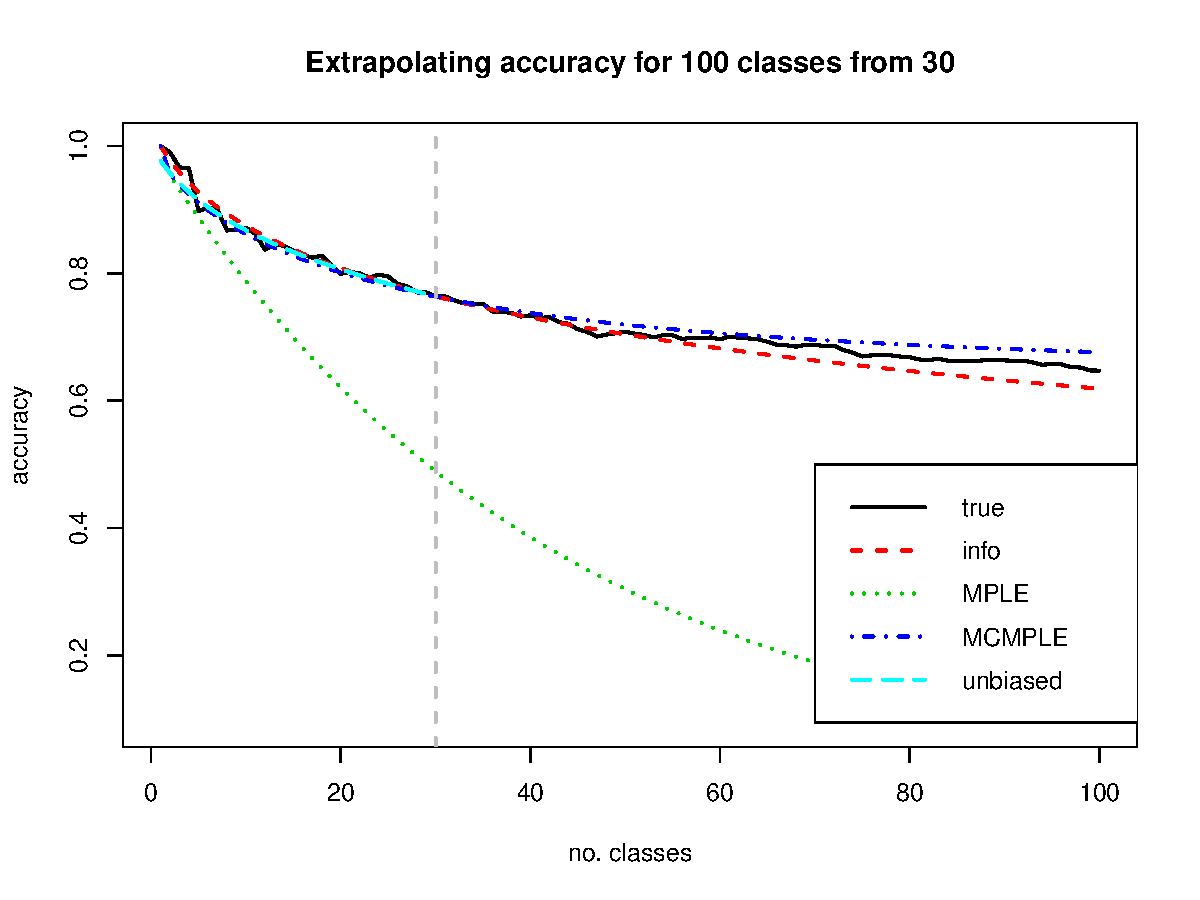
\includegraphics[scale = 0.6]{cifar_example.pdf}
\caption{Extrapolation classification performance for CIFAR data.  (This simulation needs to be fixed later.)
PMLE: maximum psuedolikelihood. MCPMLE: Moment-constrained max psuedolikelihood.  Info: Zheng and Benjamini's info-theoretic method.
Unbiased: U-statistic (cannot be used to extrapolate.) }
\end{figure}

\section{Discussion}


\subsubsection*{Acknowledgments}

CZ is supported by an NSF graduate research fellowship.

\section*{References}

\small

[X] Naselaris, T., Kay, K. N., Nishimoto, S., \& Gallant,
J. L. (2011). Encoding and decoding in fMRI. \emph{Neuroimage}, 56(2),
400-410.

[X] Friedman, Jerome, Trevor Hastie, and Robert Tibshirani. \emph{The elements
of statistical learning.} Vol. 1. Springer, Berlin: Springer series in
statistics, 2008.

\end{document}
